\section{Usability}
In their current state, unikernels are not as usable as docker containers. Docker, or container technology in general, has a working abstraction between code and infrastructure. Unikernels currently lack that abstraction. If a unikernel supports a certain language, then the application code should also be in that language. MirageOS is writen supports OCaml, and all the libraries are also written in OCaml. That makes it really hard for someone to develop applications if they are not familiar with the language. This makes in sense that application code blends in perfectly with the operating system it's being built into, nevertheless it restricts developers to develop programs in broad sense.

The networking in unikernels is not as easy to use as in docker containers. Docker containers are processes and connecting processes through ports is a well established in computer engineering. Unikernels have their own networking stack for each hypervisor and they are not unified. Bonk et al. \cite{Bonk} explains how certain networking stacks are implemented in MirageOS and how they differ from each other.

On the other hand, there are projects where MirageOS was used for superior functionality. An example project is called Jitsu\cite{jitsu}, Just in time summoning of unikernels. In that project, for every DNS request they are starting a unikernel to respond to that request. The working principle can be seen in \ref{fig:jitsu}.

\begin{figure}[htpb]
    \centering
    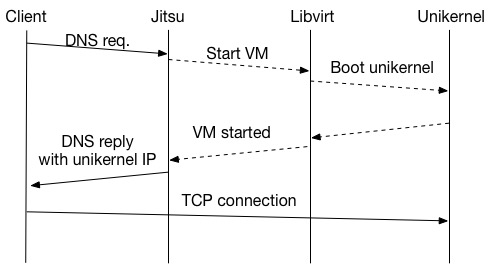
\includegraphics[width=0.8\textwidth]{figures/jitsu.jpg}
    \caption{Jitsu \cite{jitsu}} \label{fig:jitsu}
  \end{figure}

This project is being used to serve static websites, which is a simple task to do. Nevertheless, their fast boot times allows them to use unikernels instead of docker containers. The DNS server running in that example is also a unikernel, so the environment can be achieved in a pure unikernel fashion.

Another unikernel stack , IncludeOS, writes it's applicatios in C++. C++ is a more industry oriented language than OCaml, but they still have the same network problems. IncludeOS requires an additional file to set up network correctly. It's also not easy to set up their hello\_world example correctly.